% Licencia: CC BY-SA 3.0

%% Paquetes y configuración %

% Beamer
\PassOptionsToPackage{unicode}{hyperref}  % Evita errores con caracteres no ASCII
\PassOptionsToPackage{naturalnames}{hyperref} % tex.stackexchange.com/questions/10555
\documentclass[compress]{beamer}

% Idioma
\usepackage[spanish]{babel} % Traducciones
\usepackage[utf8]{inputenc} % Uso de caracteres UTF-8
\usepackage{lmodern}        % Fuentes de tamaño arbitrario
\usepackage[T1]{fontenc}    % Permite copiar y evita errores
\uselanguage{Spanish}       % Traducciones beamer
\languagepath{Spanish}      % (tex.stackexchange.com/questions/168208)

% Matemáticas
\usepackage{amsfonts}
\usepackage{amsmath}
\usepackage{amssymb}
\usepackage{mathrsfs}
\usepackage{xfrac}
\newtheorem*{proposicion}{Proposición}
\newtheorem*{teorema}{Teorema}
\theoremstyle{definition}
\newtheorem*{definicion}{Definición}
\newtheorem*{problema}{Problema}
\theoremstyle{remark}
\newtheorem*{solucion}{Solución}

% Colores
\definecolor{backg}{HTML}{F2F2F2}    % Fondo
\definecolor{title}{HTML}{bdc3d1}    % Títulos
\definecolor{comments}{HTML}{BDBDBD} % Comentarios
\definecolor{keywords}{HTML}{08388c} % Palabras clave
\definecolor{strings}{HTML}{FA5858}  % Strings
\definecolor{links}{HTML}{2C2C95}    % Enlaces
\definecolor{bars}{HTML}{045FB4}     % Barras (gráfico)

% Código
\usepackage{listings}
\lstset{
language=Octave,
basicstyle=\footnotesize,
breaklines=true,
backgroundcolor=\color{backg},
keywordstyle=\color{keywords},
commentstyle=\color{comments},
stringstyle=\color{strings},
tabsize=2,
% Acentos, ñ, ¿, ¡ (tex.stackexchange.com/questions/24528)
extendedchars=true,
literate={á}{{\'a}}1 {é}{{\'e}}1 {í}{{\'i}}1 {ó}{{\'o}}1
         {ú}{{\'u}}1 {ñ}{{\~n}}1 {¡}{{\textexclamdown}}1
         {¿}{{?`}}1
}

% Gráficos
\usepackage{tikz}
\usetikzlibrary{arrows}
\usetikzlibrary{decorations.markings}

%% Temas %%
% Tema y tema de color
  \usetheme{Dresden}
  \usecolortheme{dolphin}
  \useinnertheme{circles}
  \setbeamercovered{transparent}
% Colores bloques
  \setbeamercolor{block title}{bg=title,fg=links}
  \setbeamercolor{block body}{bg=backg,fg=black}
  \setbeamercolor{block title alerted}{fg=red!70!black,bg=title!92!red}
  \setbeamercolor{block body alerted}{fg=black,bg=backg}
  \setbeamercolor{block title example}{fg=green!70!black,bg=title!92!green}
  \setbeamercolor{block body example}{fg=black,bg=backg}
% Enlaces (tex.stackexchange.com/questions/13423)
\hypersetup{colorlinks,linkcolor=,urlcolor=links}
% Quita enlaces de navegación (stackoverflow.com/questions/3017030)
\setbeamertemplate{navigation symbols}{}
% Quita barra inferior (stackoverflow.com/questions/1435837)
\setbeamertemplate{footline}{}
% Evita warnings boxes
\hfuzz=20pt
\vfuzz=20pt
% Evita warnings itemize
\renewcommand\textbullet{\ensuremath{\bullet}}

%% Título y otros %%
\title{Interpolación con splines cuadráticos} % Título
\subtitle{Métodos Numéricos}                  % Subtítulo
% Autores (tex.stackexchange.com/questions/63259)
\author[Rubén M. \and Pablo B. \and Francisco M. \and Pablo M.\and Miguel A.]
{\texorpdfstring{
  \begin{columns}
    \column{.2\linewidth}
    \centering
    Rubén Morales \\
    \column{.2\linewidth}
    \centering
    Pablo Baeyens \\
    \column{.2\linewidth}
    \centering
    Francisco Morales \\
    \column{.2\linewidth}
    \centering
    Pablo Medina \\
    \column{.2\linewidth}
    \centering
    Miguel Anguita \\
  \end{columns}
}{
Rubén Morales \and Pablo Baeyens \and Francisco Morales
\and Pablo Medina \and Miguel Anguita
}}

\date{10 de Junio de 2015} % Fecha



%% Presentación %%
\begin{document}

\begin{frame}
\titlepage
\end{frame}

\section{Introducción}

\begin{frame}{Splines cuadráticos}
\begin{definicion}
Un \textbf{spline cuadrático} es una función $s \in S_2^1(P)$, para
cierta partición $P$ sobre un intervalo.
\end{definicion}
\begin{columns}
\column{0.5\textwidth}
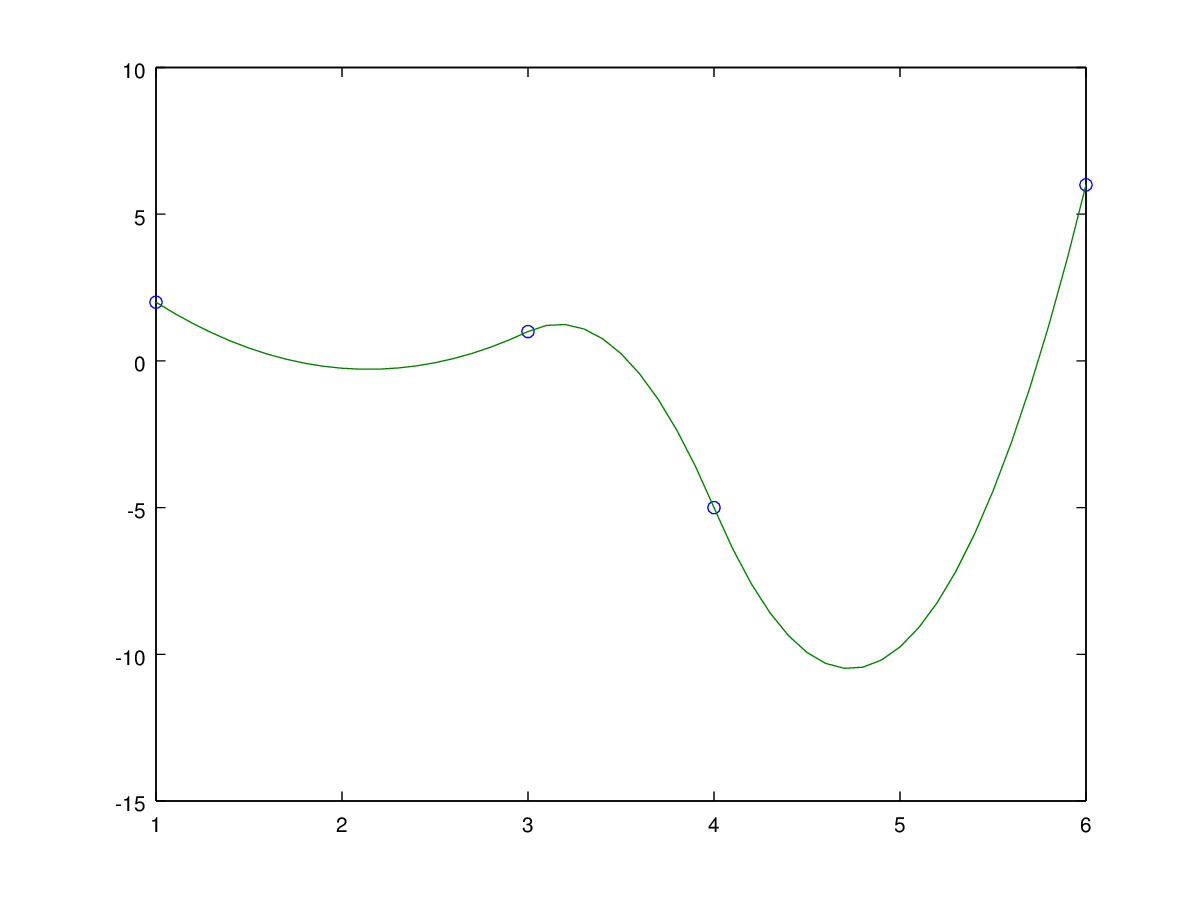
\includegraphics[width=\textwidth]{EjemploDef.png}
\column{.5\textwidth}
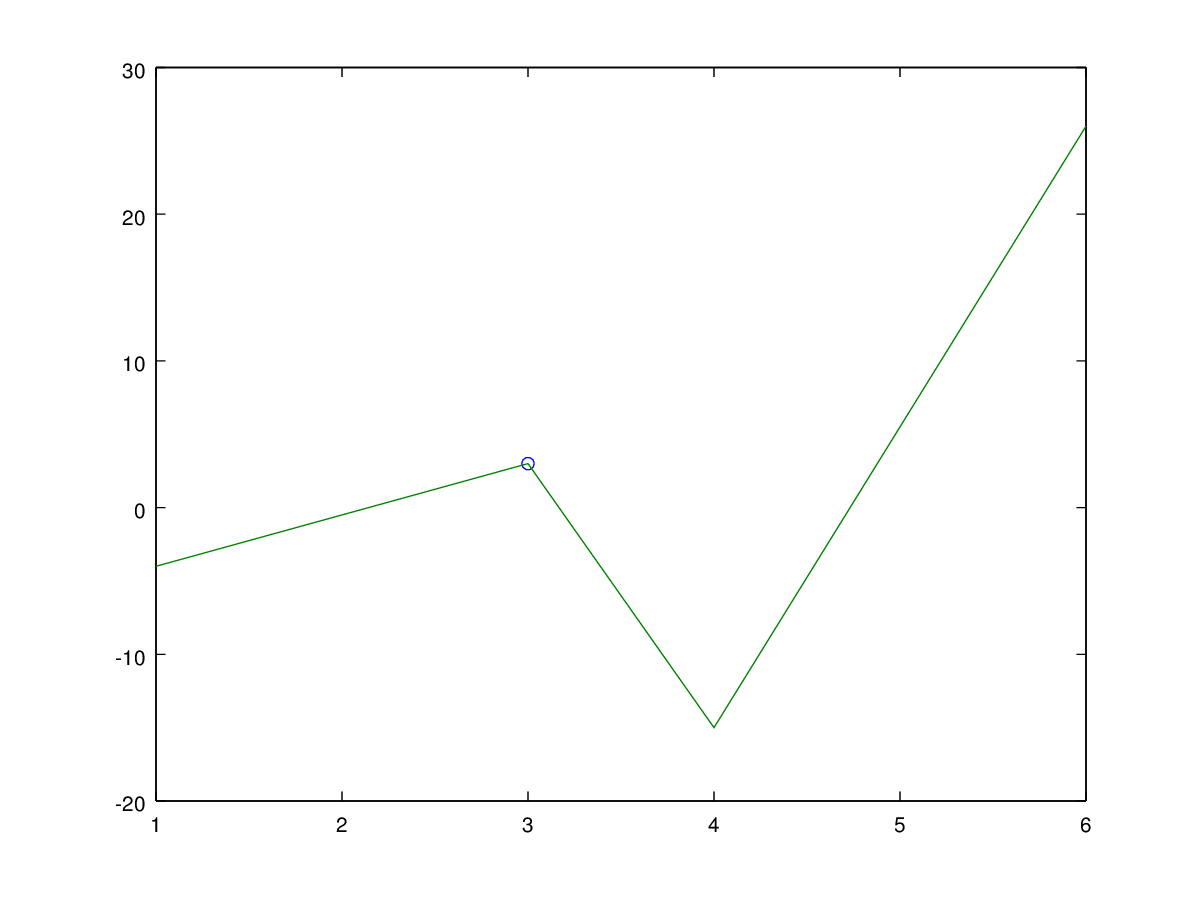
\includegraphics[width=\textwidth]{EjemploDefDer.png}
\end{columns}
\end{frame}

\begin{frame}{Dimensión del espacio}
\begin{proposicion}
Sea $[a,b]$ intervalo, $P = \{x_i\}_{i=0...\alert<1>{n}} \in \mathscr{P}([a,b])$,
entonces $\dim(S_2(P)) = \alert<2>{n+2}$.
\end{proposicion}
\begin{proof}<3->
Podemos deducirlo a partir de la fórmula general:

\[
\dim(S_{\alert<4>{k}}^{\alert<5>{r}}(P)) = (\alert<4>{k} - \alert<5>{r})n
+ \alert<5>{r} + 1
\]

Así:

\[\dim(S_{\alert<4>{2}}^{\alert<5>{1}}(P)) = (\alert<4>{2} - \alert<5>{1})n + \alert<5>{1} + 1 = 2\]
\end{proof}
\end{frame}

\begin{frame}{Base del espacio}
\begin{block}{Base}
Conocida la dimensión podemos establecer una base:
\[\{1, x, x^2, (x-x_1)_+^2, ... , (x-x_{n-1})_+^2\}\]
\end{block}
\end{frame}

\section{Interpolación}

\begin{frame}{Método local}
Dada la derivada en el nodo $k$, podemos calcular mediante
diferencias divididas los trozos a ambos lados:

\vfill

\begin{overlayarea}{\textwidth}{.4\textheight}
\only<1>{
Si $d_k$ queda a la \textbf{derecha} del trozo:
\begin{table}[h]
\centering
\begin{tabular}{llll}
$x_{k-1}$ & $y_{k-1}$ & & \\
$x_k$ & $y_k$ & $p_k$ & \\
$x_k$ & $y_k$ & $d_k$ & $\frac{d_k-p_k}{h_k}$
\end{tabular}
\end{table}

\begin{equation} \label{eq:sk}
s_k(x)=y_{k-1}+p_k(x-x_{k-1})+\frac{d_k-p_k}{h_k}(x-x_{k-1})(x-x_k)
\end{equation}

}

\only<2>{
Si $d_k$ queda a la \textbf{izquierda} del trozo:
\begin{table}[h]
\centering
\begin{tabular}{llll}
$x_k$ & $y_k$ & & \\
$x_k$ & $y_k$ & $d_k$ & \\
$x_{k+1}$ & $y_{k+1}$ & $p_{k+1}$ & $\frac{p_{k+1}-d_k}{h_k}$
\end{tabular}
\end{table}

\begin{equation} \label{eq:skmas}
s_{k+1}(x)=y_k+d_k(x-x_k)+\frac{p_{k+1}-d_k}{h_{k+1}}(x-x_k)(x-x_k)
\end{equation}

}
\end{overlayarea}
\end{frame}

\begin{frame}{Método local}

Repetimos este proceso actualizando la derivada:

\begin{itemize}
\item Hacia la \alert<1>{izquierda}, aplicando la primera fórmula.
\item Hacia la \alert<2>{derecha}, aplicando la segunda fórmula.
\end{itemize}

\vfill

\begin{tikzpicture}[scale=1.5]
\draw (-3.5,0) -- (-2.5,0);
\draw[dotted] (-2.5, 0) -- (-1.5,0);
\draw (-1.5,0) -- (1.5,0);
\draw[dotted] (1.5, 0) -- (2.5,0);
\draw (2.5,0) -- (3.5,0);

\foreach \x in  {-3,-1,0,1,3}
\draw[shift={(\x,0)},color=black] (0pt,3pt) -- (0pt,-3pt);

\draw[shift={(1,0)},color=black] (0pt,0pt) -- (0pt,-3pt)
node[below] {$x_{k+1}$};
\draw[shift={(-1,0)},color=black] (0pt,0pt) -- (0pt,-3pt)
node[below] {$x_{k-1}$};
\draw[shift={(0,0)},color=black] (0pt,0pt) -- (0pt,-3pt)
node[below] {$x_k$};
\draw[shift={(-3,0)},color=black] (0pt,0pt) -- (0pt,-3pt)
node[below] {$x_0$};
\draw[shift={(3,0)},color=black] (0pt,0pt) -- (0pt,-3pt)
node[below] {$x_n$};

\draw (0.5,0) edge[ultra thin, ->, bend left=50, looseness=1]  node[above right] {\alert<2>{\footnotesize $d_{k+1} = s'_k(x_{k+1})$}} (2,0.15);
\draw (-0.5,0) edge[ultra thin, ->, bend right=50, looseness=1]  node[above left] {\alert<1>{\footnotesize $d_{k-1} = s'_k(x_{k-1})$}} (-2,0.15);
\end{tikzpicture}
\end{frame}

\begin{frame}{Método global}

Resolvemos el sistema, añadiendo la condición para la derivada:

\begin{equation*}
\begin{pmatrix}
  1 & x_0 & x_0^2   & 0 & \cdots & 0\\
  1 & x_1 & x_1^2   & (x_1-x_1)_{+}^2 & \cdots & 0\\
  \vdots& & \vdots  & \vdots          & \cdots & \vdots \\
  \vdots& & \vdots  & \vdots          & \cdots & \vdots \\
  1 & x_n & x_n^2   & (x_n-x_1)_{+}^2 & \cdots & (x_n-x_{n-1})_{+}^2\\
  \alert<2>{0} &   \alert<2>{1} &  \alert<2>{2x_k} & \alert<2>{2(x_k-x_1)_{+}} & \alert<2>{\cdots} & \alert<2>{2(x_k-x_{n-1})_{+}}
\end{pmatrix}
\begin{pmatrix}
  a \\
  b \\
  c \\
  \alpha_1 \\
  \vdots \\
  \alpha_{n-1}
\end{pmatrix}
=
\begin{pmatrix}
  y_0\\
  y_1\\
  \vdots\\
  \vdots\\
  y_n\\
  \alert<2>{d_k}\\
\end{pmatrix}
\end{equation*}

\vspace{2pt}

\uncover<3>{
\begin{equation*}
 s(x) = a + bx + cx^2 + \alpha_1(x-x_1)_+^2 + \cdots + \alpha_{n-1}(x-x_{n-1})_+^2
\end{equation*}
}
\end{frame}

\section{Implementación}

\begin{frame}[fragile]{\texttt{SplineCuad}}
Implementamos la función con el \textbf{método global}.
\begin{enumerate}[<only@+>]
\item Calculamos la matriz de coeficientes:
\begin{lstlisting}
n = length(x) - 1;

A(:,1) = [ones(n+1,1); 0];
A(:,2) = [x'         ; 1];
A(:,3) = [x'.^2      ; 2.*x(k+1)];

for j = 4 : n + 2
  t       =  @(s) (s > x(j-2)) .* (s - x(j-2));
  A(:, j) = [t(x').^2; 2.*t(x(k+1))];
end
\end{lstlisting}

\item Y resolvemos el sistema:
\begin{lstlisting}
sol = A \ [y' ; d_k];

for k = 1:n
  p = sol(3:-1:1)';

  for l = 2:k
    p += sol(l+2).*[1, -2.*x(l), x(l).^2];
  end

  B(k, :) = polyaffine(p,[-x(k) 1]);
end

s = mkpp(x,B);
\end{lstlisting}
\end{enumerate}
\end{frame}

\begin{frame}[fragile]{\texttt{SplineCuadLocal}}
\begin{enumerate}[<only@+>]

\item Recorremos todos los nodos de \texttt{k+1} en adelante:
\begin{lstlisting}
for i = (k+1):(length(x)-1)
  p = (y(i+1)-y(i))/(x(i+1)-x(i));
  q = (p-d)/(x(i+1)-x(i));
  v = [x(i) x(i)];
  s(i,:) = [0, 0, y(i)]+[0, d, -d*x(i)]+q*poly(v);
  d = polyval(polyder(s(i,:)),x(i+1));
end
  d = d_k;
\end{lstlisting}

\item Recorremos todos los nodos desde \texttt{k} hasta el \texttt{1}:
\begin{lstlisting}
for j = k:-1:1
  p = (y(j+1)-y(j))/(x(j+1)-x(j))
  q = (d-p)/(x(j+1)-x(j))
  v = [x(j) x(j+1)]
  s(j,:) = [0 0 y(j)]+[0 p -p*x(j)]+q*poly(v);
  d = polyval(polyder(s(j,:)), x(j))
end
\end{lstlisting}

\item Y cambiamos de base usando \texttt{polyaffine}:
\begin{lstlisting}
for i = 1:length(s)
  s(i,:) = polyaffine(s(i,:), [-x(i), 1]);
end
\end{lstlisting}
\end{enumerate}
\end{frame}

\end{document}
